% Measure-AI-Drift Thesis
% Bachelor's Thesis: LLM Stability in Therapeutic Contexts
%
% Compile with: latexmk -pdf main.tex
% Or: pdflatex main.tex && biber main && pdflatex main.tex && pdflatex main.tex

\documentclass[11pt,
  paper=a4,
  bibliography=totocnumbered,
  captions=tableheading,
  BCOR=10mm
]{scrreprt}

% --- Encoding and fonts ---
\usepackage[utf8]{inputenc}
\usepackage[T1]{fontenc}
\usepackage{lmodern}

% --- Language ---
\usepackage[english]{babel}

% --- Spacing ---
\usepackage[onehalfspacing]{setspace}

% --- Quoting ---
\usepackage{csquotes}

% --- Math ---
\usepackage{amsmath}
\usepackage{amsthm}
\usepackage{amssymb}
\usepackage{mathtools}

% --- Floats and figures ---
\usepackage[section]{placeins}
\usepackage{graphicx}
\usepackage{subcaption}
\usepackage{floatrow}
\floatsetup[table]{style=plaintop}
\graphicspath{{figures/}{../visualizations/}}

% --- Tables ---
\usepackage{booktabs}
\usepackage{tabularx}
\usepackage{multirow}

% --- Typography ---
\usepackage[all]{nowidow}

% --- Hyperlinks ---
\usepackage[
  colorlinks=true,
  linkcolor=black,
  citecolor=blue!60!black,
  urlcolor=blue!70!black
]{hyperref}

% --- Code listings ---
\usepackage{xcolor}
\usepackage{listings}
\lstset{
  basicstyle=\ttfamily,
  keywordstyle=\color{black}\bfseries\underbar,
  identifierstyle=,
  commentstyle=\color{white},
  stringstyle=\ttfamily,
  showstringspaces=false,
  numbers=left,
  numberstyle=\tiny,
  stepnumber=1
}

% JSON syntax highlighting
\colorlet{json:punct}{red!60!black}
\colorlet{json:numb}{magenta!60!black}
\definecolor{json:delim}{RGB}{20,105,176}
\lstdefinelanguage{json}{
  basicstyle=\linespread{0.9}\ttfamily,
  showstringspaces=false,
  breaklines=true,
  breakindent=4pt,
  breakautoindent=false,
  literate=
   *{0}{{{\color{json:numb}0}}}{1}
    {1}{{{\color{json:numb}1}}}{1}
    {2}{{{\color{json:numb}2}}}{1}
    {3}{{{\color{json:numb}3}}}{1}
    {4}{{{\color{json:numb}4}}}{1}
    {5}{{{\color{json:numb}5}}}{1}
    {6}{{{\color{json:numb}6}}}{1}
    {7}{{{\color{json:numb}7}}}{1}
    {8}{{{\color{json:numb}8}}}{1}
    {9}{{{\color{json:numb}9}}}{1}
    {:}{{{\color{json:punct}{:}}}}{1}
    {,}{{{\color{json:punct}{,}}}}{1}
    {\{}{{{\color{json:delim}{\{}}}}{1}
    {\}}{{{\color{json:delim}{\}}}}}{1}
    {[}{{{\color{json:delim}{[}}}}{1}
    {]}{{{\color{json:delim}{]}}}}{1},
}

% Python syntax highlighting
\definecolor{py:keyword}{RGB}{0,128,0}
\definecolor{py:string}{RGB}{186,33,33}
\definecolor{py:comment}{RGB}{128,128,128}
\lstdefinestyle{python}{
  language=Python,
  basicstyle=\linespread{0.9}\ttfamily\small,
  keywordstyle=\color{py:keyword}\bfseries,
  stringstyle=\color{py:string},
  commentstyle=\color{py:comment}\itshape,
  showstringspaces=false,
  breaklines=true,
  numbers=left,
  numberstyle=\tiny\color{gray},
}

% --- Colored boxes (for prompt examples, model outputs) ---
\usepackage[skins,breakable]{tcolorbox}
\tcbset{boxrule=0.5pt}

% --- Bibliography (APA style for psychology-adjacent thesis) ---
\usepackage[
  backend=biber,
  style=apa,
  sorting=nyt
]{biblatex}
\addbibresource{references.bib}

% --- Glossary and acronyms ---
\usepackage[automake, nopostdot, nonumberlist]{glossaries}
\makeglossaries

% --- Misc ---
\usepackage{authoraftertitle}

%%% Custom commands %%%

% Model names in small caps
\newcommand{\modelname}[1]{\textsc{#1}}

% Inline code
\newcommand{\codeil}[1]{\lstinline{#1}}{}
\newcommand{\techil}[1]{\texttt{#1}}

% Shorthands
\newcommand{\ie}{i.\,e.~}
\newcommand{\eg}{e.\,g.~}
\newcommand{\vs}{vs.~}

% Reference helpers
\newcommand{\figref}[1]{(cf.~Figure \ref{#1})}
\newcommand{\figureref}[1]{Figure \ref{#1}}
\newcommand{\tabref}[1]{(cf.~Table \ref{#1})}
\newcommand{\tableref}[1]{Table \ref{#1}}

% Figure width
\def \figwidth {0.9\linewidth}

% Capitalized autoref names
\renewcommand*{\chapterautorefname}{Chapter}
\renewcommand*{\sectionautorefname}{Section}

% Signature line for declaration
\newcommand{\namesigdate}[1][5cm]{%
  \vspace{5cm}
  {\setlength{\parindent}{0cm}
  \begin{minipage}{0.3\textwidth}
    \hrule
    \vspace{0.5cm}
    {\small city, date}
  \end{minipage}
  \hfill
  \begin{minipage}{0.3\textwidth}
    \hrule
    \vspace{0.5cm}
    {\small signature}
  \end{minipage}
  }
}

%%% Acronym definitions %%%
\newacronym{llm}{LLM}{Large Language Model}
\newacronym{irt}{IRT}{Imagery Rehearsal Therapy}
\newacronym{moe}{MoE}{Mixture of Experts}
\newacronym{eu}{EU}{European Union}
\newacronym{api}{API}{Application Programming Interface}
\newacronym{json}{JSON}{JavaScript Object Notation}
\newacronym{cbt}{CBT}{Cognitive Behavioral Therapy}
\newacronym{rlhf}{RLHF}{Reinforcement Learning with Human Feedback}
\newacronym{gdpr}{GDPR}{General Data Protection Regulation}
\newacronym{ptsd}{PTSD}{Post-Traumatic Stress Disorder}
\newacronym{cot}{CoT}{Chain-of-Thought}
\newacronym{nli}{NLI}{Natural Language Inference}
\newacronym{bdi}{BDI}{Brief Dreamer Interview}
\newacronym{nlp}{NLP}{Natural Language Processing}

%%% Document metadata %%%
\title{Measuring Drift in Therapeutic AI: A Stability-Based Evaluation of Sovereign LLMs in Nightmare Therapy}
\author{Daniel Menzel}
\date{\today}

\begin{document}

% --- Title page ---
\begin{titlepage}
  \begin{flushleft}
    Universit\"at Osnabr\"uck\\
    Fachbereich Humanwissenschaften\\
    Institute of Cognitive Science
  \end{flushleft}

  \vspace{2cm}
  \centering{
    Bachelor's Thesis\vspace{1cm}\\
    \textbf{\Large{\MyTitle}}
    \vspace{1cm}\\
    \begin{tabular}{c}
      \MyAuthor                             \\
      979 379                               \\
      Bachelor's Program Cognitive Science  \\
      Winter 2025/2026
    \end{tabular}}
  \vspace{1cm}

  \begin{tabular}{ll}
    First supervisor:  & Moritz Hartstang                \\
                       & Institute of Cognitive Science  \\
                       & Osnabr\"uck                     \\\\
    Second supervisor: & Prof.\ Dr.\ Sebastian Musslick  \\
                       & Institute of Cognitive Science  \\
                       & Osnabr\"uck
  \end{tabular}

\end{titlepage}


% --- Declaration of Authorship ---
\chapter*{Declaration of Authorship}
The content of this thesis represents my own knowledge, my own understanding and my own perspective on the topic.
In case artificial intelligence tools were used, their way and purpose of usage has been made transparent.
Moreover, I have cited all my sources in accordance with academic standards.
I am ready and able to explain and defend the positions developed in this thesis.
This thesis has not been submitted, either in part or whole, at this or any other university.

\namesigdate
\pagenumbering{gobble}
\pagebreak


% --- Abstract ---
\begin{abstract}
  \textbf{\LARGE{Abstract}}\\\\
  Large language models are increasingly used as therapeutic agents in
  mental health applications, but it is unclear how consistently they
  respond when given the same patient input multiple times. This thesis
  measures therapeutic stability in the rescripting phase of Imagery
  Rehearsal Therapy, where the model must choose a therapeutic strategy
  and generate a response that carries it out.

  Ten models, including the EU-sovereign Mistral Large~3, two proprietary
  models (GPT-5.4, Claude Sonnet~4.6), and seven open-weight comparators,
  are evaluated across 6{,}000 trials at five temperature settings. A
  three-level evaluation framework compares strategy selections (Jaccard
  similarity), response texts (BERTScore), and whether the model does what
  it declared (LLM judge alignment).

  The main findings are: (1)~Mistral Large~3 matches the proprietary
  models on plan consistency at its recommended temperature range.
  (2)~Temperature affects which strategies the model picks but not how
  well it carries them out. The instability sits in strategy selection,
  not in response quality. (3)~Greedy decoding ($T = 0.0$) is not
  optimal for all models; three achieve higher consistency at $T = 0.075$.
  (4)~BERTScore captures whether the therapeutic tone stays similar but
  does not detect changes in the underlying strategy. The three levels
  together reveal patterns that no single metric shows on its own.

  At low temperatures, the EU-sovereign Mistral Large~3 reaches the same
  plan consistency as the proprietary models. At higher temperatures, the
  proprietary models remain stable while Mistral degrades. The framework
  itself is not specific to IRT and could be applied to other structured
  therapy protocols.
\end{abstract}


% --- Lists ---
\tableofcontents
\listoffigures
\listoftables


% --- Main matter ---
\pagenumbering{arabic}

\chapter{Introduction}
\label{chap:introduction}

\section{Nightmare Disorder and Imagery Rehearsal Therapy}
\label{sec:intro-irt}
% ~5% prevalence, comorbidity with PTSD/depression
% IRT as gold-standard: structured protocol with rescripting at its core
% Clinician shortage -> scalable AI interventions as potential solution

\section{AI-Assisted Psychotherapy}
\label{sec:intro-ai-therapy}
% LLM-based therapeutic delivery (reDreamAI project as applied context)
% Distinction: general-purpose conversational AI vs. protocol-driven therapeutic agents
% Deployment in clinical settings introduces regulatory constraints (EU AI Act, data sovereignty)

\section{The Evaluation Gap}
\label{sec:intro-eval-gap}
% Standard NLP benchmarks do not assess therapeutic reliability
% Missing: intent stability under stochastic variation, protocol adherence, consistent persona
% Need for domain-specific in silico clinical trials

\section{Research Objectives}
\label{sec:intro-objectives}
% RQ: How consistent is LLM clinical reasoning across stochastic runs in a structured therapeutic protocol?
% Contribution 1: Three-level hierarchical evaluation framework for therapeutic AI stability
% Contribution 2: Quantitative comparison across model classes (sovereign, proprietary, open-weight)
% Scope: isolated rescripting phase (cognitive core of IRT)

\chapter{Background}
\label{chap:background}

\section{Imagery Rehearsal Therapy}
\label{sec:bg-irt}
% Five-stage IRT protocol: recording -> rewriting -> summary -> rehearsal -> final
% The rescripting phase as the core cognitive intervention
% Clinical evidence and treatment fidelity assessment in psychotherapy

\section{Large Language Models in Healthcare}
\label{sec:bg-llm-healthcare}
% Current therapeutic AI applications and their evaluation
% Challenges in high-stakes settings: hallucination, drift, inconsistency
% Regulatory landscape: EU AI Act, Medical Device Regulation

\section{Stochastic Behaviour in Language Models}
\label{sec:bg-stochastic}
% Temperature-based sampling and output variance
% Reproducibility challenges across repeated generations
% Prior work on measuring LLM behavioural stability and drift

\section{Evaluation Metrics for Text Generation}
\label{sec:bg-metrics}
% Traditional metrics (BLEU, ROUGE) and their limitations for semantic comparison
% BERTScore: contextual embedding-based evaluation (Zhang et al., 2020)
% LLM-as-judge: paradigm, known biases, mitigation strategies

\section{Chain-of-Thought and Plan Faithfulness}
\label{sec:bg-cot}
% CoT prompting (Wei et al., 2022)
% Faithfulness concerns: CoT as post-hoc rationalisation (Turpin et al., 2023; Lanham et al., 2023)
% Implications for structured plan mechanisms in evaluation

\chapter{Methods}
\label{chap:methods}

\section{System Overview}
\label{sec:meth-overview}
% Two-stack architecture: generation stack (dialogue creation) and evaluation stack (stability measurement)
% Data flow: vignettes -> generation -> frozen histories -> evaluation -> aggregation
% Key design principle: separate dialogue creation from stability testing

\section{Dialogue Generation}
\label{sec:meth-dialogue}
% Three-agent loop: Patient (BDI-profiled vignette), Router (stage classification), Therapist (stage-appropriate response)
% Six patient vignettes: anxious, avoidant, cooperative, resistant, skeptic, trauma
% Five-stage IRT protocol traversal

\section{Frozen History Design}
\label{sec:meth-frozen}
% Deterministic evaluation entry points: identical context for every trial
% Conversation slicing at rewriting-turn boundaries (slice_1, slice_2, slice_3)
% Rationale: evaluate at different conversation depths within the rescripting phase

\section{Evaluation Stack}
\label{sec:meth-eval}
% Router bypass: rescripting prompt injected directly (stage is known a priori)
% Fused CoT generation: plan and response in a single call
%   <plan> block declares 1-2 strategies before the therapeutic response
%   Plan conditions the response tokens (Chain-of-Thought style)
% 10 independent trials per condition

\section{The Plan Mechanism}
\label{sec:meth-plan}
% Plan as declared intent, not as explanation of internal reasoning
% Structured measurement independent of CoT faithfulness debate
% Enables: strategy-level consistency measurement, alignment verification, clinical oversight
% Fixed IRT strategy taxonomy constrains output to therapeutic domain

\section{Strategy Taxonomy Development}
\label{sec:meth-taxonomy}
% Initial 8-category taxonomy: severe distribution skew (empowerment/mastery = 87.7%)
% Revision 1, merge to agency: failed (100% dominance, goal vs. mechanism confusion)
% Revision 2, mechanism-specific split: confrontation vs. self_empowerment
% Final 7 categories: confrontation, self_empowerment, safety, cognitive_reframe,
%   emotional_regulation, social_support, sensory_modulation
% Prompt-level steering for category diversity

\section{Evaluation Metrics}
\label{sec:meth-metrics}

\subsection{Method 1: Cognitive Stability (Plan Consistency)}
\label{sec:meth-m1}
% Pairwise Jaccard similarity over strategy sets: J(A,B) = |A n B| / |A u B|
% Mean over C(10,2) = 45 trial pairs
% Strategy extraction from <plan> blocks. Validity rate as quality gate
% Measures: do stochastic runs produce the same therapeutic decisions?

\subsection{Method 2: Output Consistency (Semantic Stability)}
\label{sec:meth-m2}
% Pairwise BERTScore F1 over response texts, mean over 45 pairs
% Embedding model: DeBERTa-XLarge-MNLI (He et al., 2021)
%   NLI fine-tuning aligns with semantic comparison task
%   Highest WMT16 correlation with human judgments (r = 0.778)
%   Disentangled attention handles surface-form variation in therapeutic language
% Measures: do stochastic runs produce therapeutically equivalent responses?

\subsection{Method 3: Plan-Output Alignment (Exploratory)}
\label{sec:meth-m3}
% LLM judge (Gemini Pro, T=0.0) with ternary scoring per declared strategy
%   0 = absent, 1 = partial, 2 = implemented
% Ternary scale grounded in clinical fidelity literature (ENACT, NIH BCC)
% Rejected alternatives: NLI cross-encoders (F1 ceiling ~0.55, task mismatch, no reasoning trace)
% Mitigations: cross-model judging, CoT justification, deterministic decoding, transparent rubric
% Measures: does the model's response implement its declared therapeutic plan?

\section{Model Selection}
\label{sec:meth-models}
% EU sovereignty as selection criterion: data protection, AI Act, open-weight licensing
% Primary subject: Mistral Large 3 (675B MoE, 41B active), EU-sovereign, Apache 2.0
% Proprietary baseline: GPT-5
% Open-weight comparisons: Llama 3.3 70B, Qwen 3 32B, Gemma 3 27B
% Selection rationale: size class diversity, provider diversity, sovereignty status

\section{Experimental Conditions}
\label{sec:meth-conditions}
% 6 vignettes x 3 slices x 10 trials x 2 temperatures (T=0.0, T=0.7) x N models
% T=0.0: deterministic baseline (greedy decoding)
% T=0.7: stochastic condition (clinical deployment temperature range)

\chapter{Implementation}
\label{chap:implementation}

\section{Software Architecture}
\label{sec:impl-architecture}
% Python async-first pipeline, config-driven via YAML
% Pydantic models for type-safe data flow
% Multi-provider LLM abstraction (OpenRouter, Google)

\section{Experiment Execution}
\label{sec:impl-execution}
% ExperimentRun orchestration with structured output
% Multi-trial sampling with parallel execution
% Output: config, frozen history, trials/, metrics.json, judgments.json

\section{Aggregation Pipeline}
\label{sec:impl-aggregation}
% Cross-experiment result collection
% Per-model, per-vignette, per-slice, per-temperature breakdowns

\chapter{Results}
\label{chap:results}

% All main results reported at slice_2 (mid-rescripting), aggregated across
% vignettes. Full per-condition tables in Appendix D.

All results are reported at the second rewriting-turn boundary
(\techil{slice\_2}), aggregated across six vignettes. Each data point
represents the mean of twenty independent trials. Full per-condition
tables appear in Appendix~D.

\section{Plan Validity and Strategy Distribution}
\label{sec:res-validity}
% Validity rates across models and temperatures -- quality gate before
%   any stability analysis
% Strategy frequency distribution: heatmap (model x strategy category)
% [GRAPH] Validity rate per model x temperature
% [GRAPH] Strategy frequency heatmap (model x category)

Before analysing stability, the plan extraction step must be validated.
A trial is valid if the model produces a well-formed plan block containing
at least one recognised strategy category. Across all 6{,}000 trials,
validity rates exceed 99\% for every model. The lowest rates belong to
\modelname{Qwen~3.5~27B} (99.3\%) and \modelname{OLMo~3.1~32B} (99.7\%).
All other models achieve 99.8\% or above. Validity does not vary
meaningfully with temperature. These rates confirm that the fused
chain-of-thought prompt reliably elicits structured plan output, and that
the subsequent stability metrics are computed over near-complete data.

% TODO: insert Fig D.6 (validity rate) reference when appendix is written

Strategy distributions vary across models (\autoref{fig:strategy-dist}).
All ten models draw from the same six-category taxonomy, but the relative
frequencies differ. \techil{Confrontation} and \techil{self\_empowerment}
dominate across most models. \modelname{GPT-5.4} and
\modelname{Sonnet~4.6} show the narrowest distributions, concentrating on
two to three categories. \modelname{Qwen~3.5~27B} and
\modelname{Llama~3.3~70B} spread selections more evenly across categories.
These distributional differences are a prerequisite for interpreting the
consistency results that follow: a model that always selects the same two
strategies will score high on Jaccard regardless of temperature, while a
model that draws from a wider repertoire has more room to vary.

\begin{figure}[t]
  \centering
  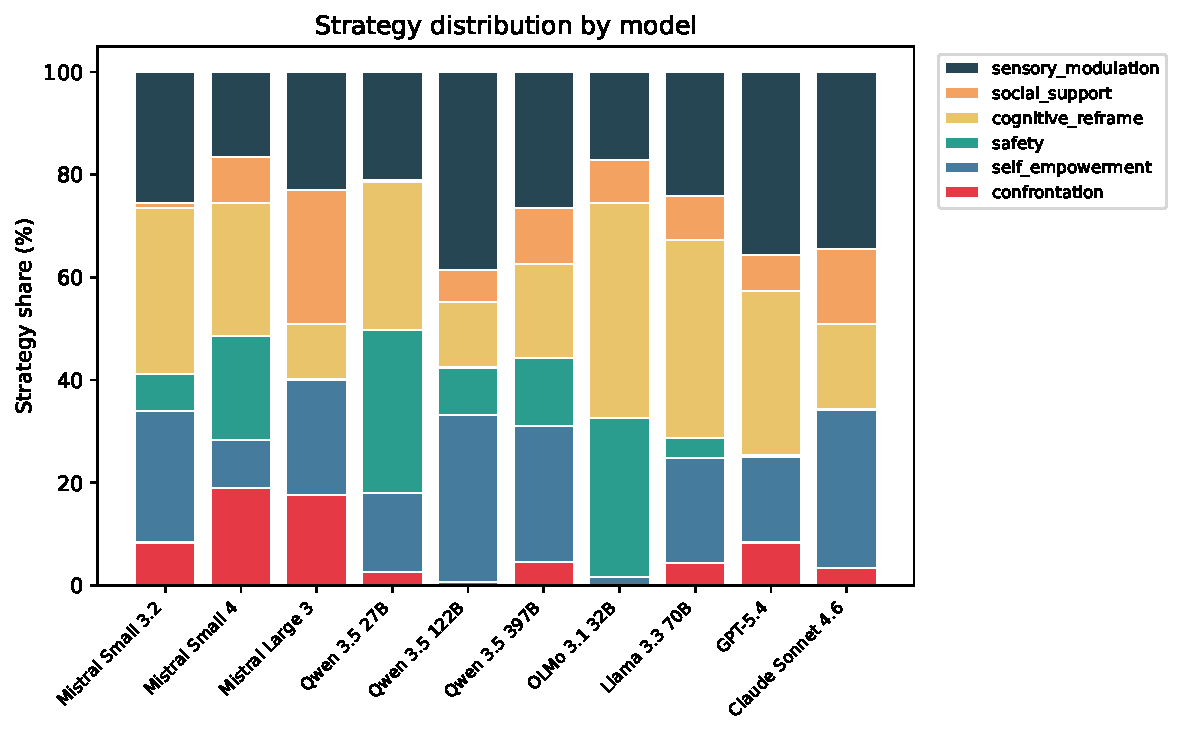
\includegraphics[width=\textwidth]{../stats/visuals_experiment/fig_5_1_strategy_distribution.pdf}
  \caption{Strategy distribution by model, pooled across temperatures and
    vignettes. Each bar shows the share of trials selecting each taxonomy
    category. Models with narrower distributions have less room to vary.}
  \label{fig:strategy-dist}
\end{figure}


% previously: Cognitive Stability (Method 1)
\section{Plan Consistency (Method 1)}
\label{sec:res-plan-consistency}
% Mean Jaccard by model x temperature -- headline figure
% Stochastic cost: degradation across temperature sweep per model
% [GRAPH] Mean Jaccard per model x temperature (bar chart)

\autoref{fig:jaccard} presents the headline result: mean Jaccard similarity
by model and temperature, grouped by model family.

\begin{figure}[t]
  \centering
  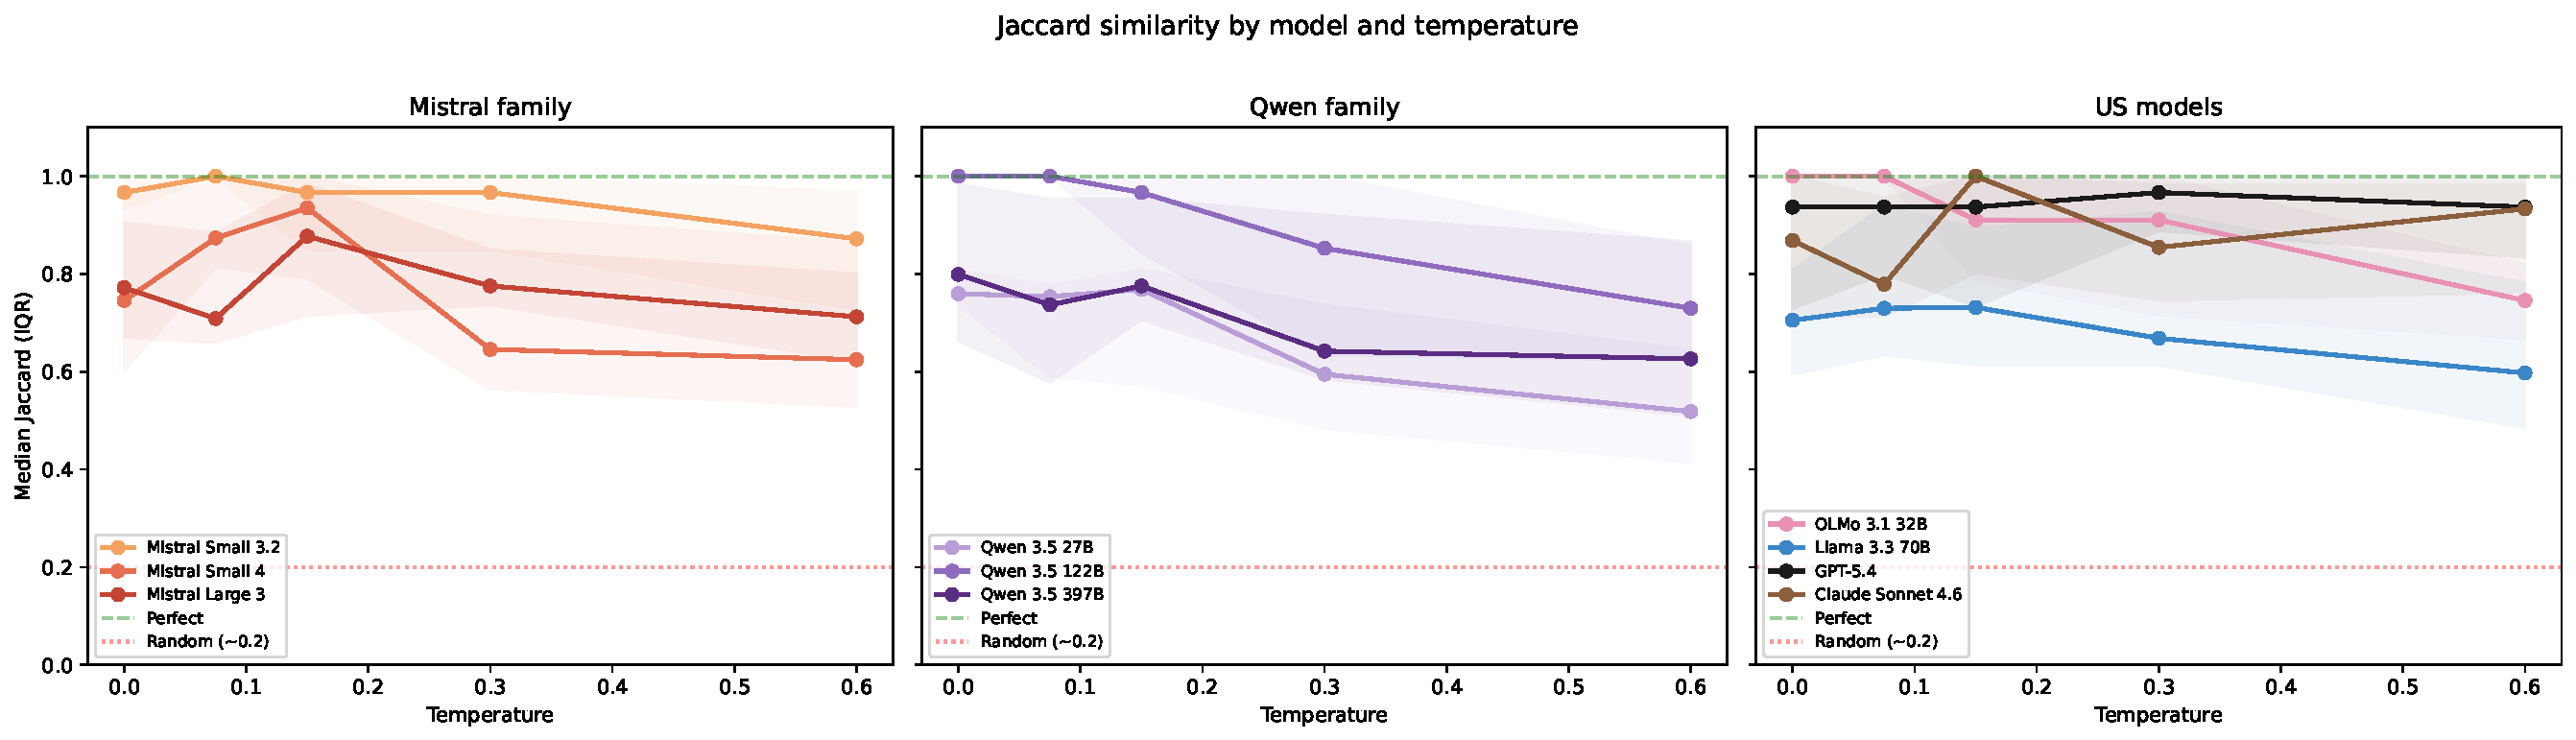
\includegraphics[width=\textwidth]{../stats/visuals_experiment/fig_5_2_jaccard.pdf}
  \caption{Mean Jaccard similarity by model and temperature, grouped by
    family. Shaded bands show $\pm 1$ SD across vignettes. The dashed
    line marks the random baseline ($J \approx 0.2$). Higher is more
    consistent.}
  \label{fig:jaccard}
\end{figure}

\paragraph{Proprietary models are temperature-immune.}
\modelname{GPT-5.4} and \modelname{Sonnet~4.6} achieve $J = 1.000$ at
every temperature point. Sampling temperature does not affect their
strategy selections at all.

\paragraph{Most open-weight models peak at low temperatures.}
The Mistral family shows a characteristic pattern:
\modelname{Mistral~Small~3.2} maintains $J = 1.000$ from $T = 0.0$
through $T = 0.3$ and drops only at $T = 0.6$ ($J = 0.933$).
\modelname{Mistral~Large~3} scores $J = 0.933$ at $T = 0.0$, rises to
$J = 1.000$ at $T = 0.075$ and $T = 0.15$, then declines to $J = 0.652$
at $T = 0.6$. \modelname{Mistral~Small~4} shows the most pronounced
version of this pattern: $J = 0.722$ at $T = 0.0$, jumping to $J = 1.000$
at $T = 0.075$ before declining.

\paragraph{Greedy decoding is not always optimal.}
Three models score higher at $T = 0.075$ than at $T = 0.0$:
\modelname{Mistral~Small~4} ($0.722 \to 1.000$),
\modelname{Mistral~Large~3} ($0.933 \to 1.000$), and
\modelname{Llama~3.3~70B} ($0.756 \to 0.881$). A small amount of sampling
variance produces more consistent strategy selection than pure greedy
decoding for these models.

\paragraph{Temperature sensitivity varies by model.}
Per-model Spearman correlations between Jaccard and temperature
(\autoref{tab:temp-spearman}) reveal three groups.
\modelname{OLMo~3.1~32B} ($\rho = -0.632$, $p < 0.001$),
\modelname{Qwen~3.5~27B} ($\rho = -0.576$, $p = 0.001$), and
\modelname{Qwen~3.5~122B} ($\rho = -0.513$, $p = 0.009$) show
statistically significant degradation. All other models, including the
entire Mistral family, show no significant temperature effect on Jaccard.
The pooled correlation across all models is $\rho = -0.228$ ($p < 0.001$).

\begin{table}[t]
  \centering
  \caption{Spearman correlation between Jaccard and temperature, per model.
    Significant correlations ($p < 0.05$) are marked with an asterisk.}
  \label{tab:temp-spearman}
  \begin{tabular}{lrrl}
    \toprule
    Model & $\rho$ & $p$ & Sig. \\
    \midrule
    Mistral Small 3.2  & $-0.190$ & 0.315 & \\
    Mistral Small 4    & $-0.196$ & 0.299 & \\
    Mistral Large 3    & $-0.277$ & 0.139 & \\
    Qwen 3.5 27B       & $-0.576$ & 0.001 & * \\
    Qwen 3.5 122B      & $-0.513$ & 0.009 & * \\
    Qwen 3.5 397B      & $-0.232$ & 0.217 & \\
    OLMo 3.1 32B       & $-0.632$ & $<$0.001 & * \\
    Llama 3.3 70B      & $-0.153$ & 0.421 & \\
    GPT-5.4            & $+0.075$ & 0.695 & \\
    Claude Sonnet 4.6  & $-0.063$ & 0.741 & \\
    \midrule
    Pooled             & $-0.228$ & $<$0.001 & * \\
    \bottomrule
  \end{tabular}
\end{table}


% previously: Output Consistency (Method 2)
\section{Response Similarity (Method 2)}
\label{sec:res-similarity}
% Mean BERTScore F1 by model x temperature -- same format as 5.2
% [GRAPH] Mean BERTScore F1 per model x temperature (bar chart)

BERTScore F1 measures semantic similarity between response texts,
independent of the plan block. The pooled temperature effect is stronger
than for Jaccard ($\rho = -0.486$, $p < 0.001$): rising temperature
changes response wording more than it changes strategy selection.

However, BERTScore has limited sensitivity to plan-level differences.
The slice depth analysis (\autoref{sec:res-secondary}) confirms this:
across conversation depths, Jaccard varies visibly while BERTScore remains
flat. A model that switches from \techil{confrontation} to
\techil{cognitive\_reframe} changes its therapeutic plan but produces
surface text similar enough that BERTScore does not detect the difference.

BERTScore therefore captures response \emph{style} consistency rather than
decision \emph{content} consistency. It serves as a sanity check: if
BERTScore were low, the model would be generating erratic text regardless
of strategy. The substantive signal for therapeutic stability comes from
Jaccard and alignment.

Full BERTScore results by model and temperature appear in Appendix~D.

% TODO: reference Fig D.2 (bertscore 3-panel) when appendix written


% previously: Plan-Output Alignment (Method 3)
\section{Plan-Response Alignment (Method 3)}
\label{sec:res-alignment}
% Mean alignment score by model x temperature
% Per-strategy scoring distributions (absent / partial / implemented)
% [GRAPH] Mean alignment per model x temperature
% [GRAPH] Stacked bar: absent / partial / implemented per strategy category

\autoref{fig:alignment} shows plan-response alignment by temperature and
per model. Alignment measures whether the model's response implements the
strategies it declared in its plan.

\begin{figure}[t]
  \centering
  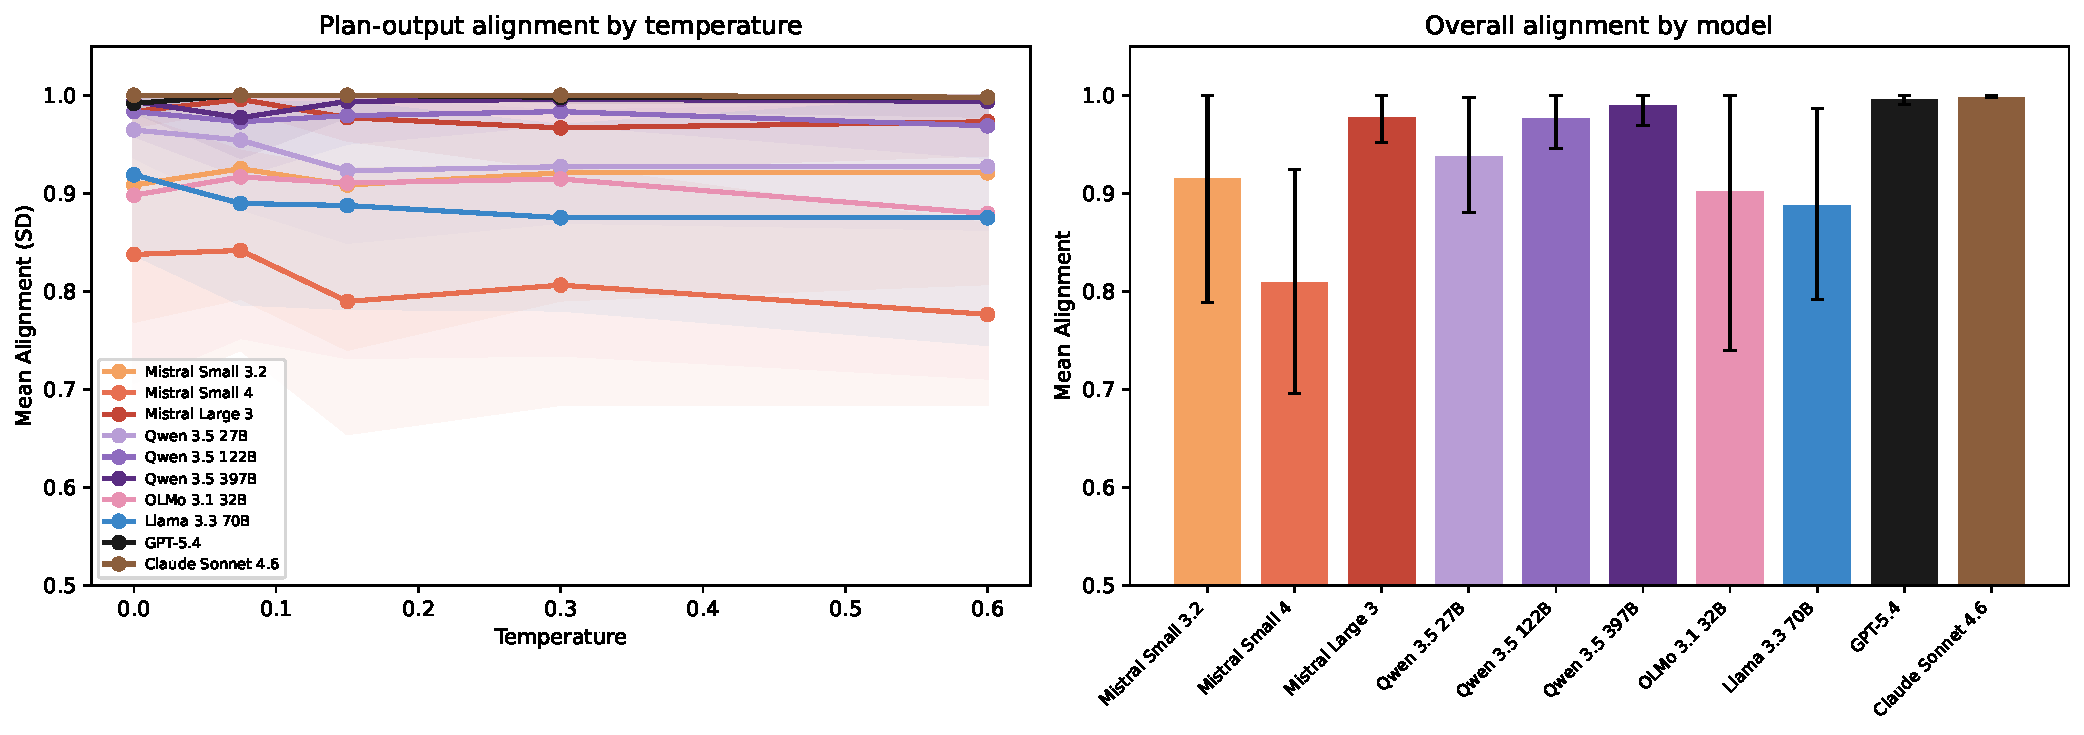
\includegraphics[width=\textwidth]{../stats/visuals_experiment/fig_5_6_alignment.pdf}
  \caption{Plan-response alignment by temperature (left) and overall by
    model (right). Error bars show $\pm 1$ SD. Most models implement their
    declared strategies consistently regardless of temperature.}
  \label{fig:alignment}
\end{figure}

The central finding is that alignment is temperature-independent. The
pooled Spearman correlation between alignment and temperature is
$\rho = -0.053$ ($p = 0.361$), not significant. Models do not get worse
at implementing their declared strategies as temperature rises. They
select \emph{different} strategies more often (lower Jaccard) but
implement whichever strategies they select equally well (stable alignment).

This dissociation has a clinical implication: temperature-induced
instability occurs at the decision-making level, not at the execution
level. A model at high temperature does not produce incoherent responses.
It produces coherent responses to a different therapeutic plan.

Kruskal-Wallis tests confirm that models differ significantly on alignment
($p < 0.001$). \modelname{Mistral~Small~4} shows the lowest mean
alignment, consistent with its erratic strategy selection at extreme
temperatures. The proprietary models and \modelname{Mistral~Small~3.2}
cluster near the top.


\section{Cross-Method Analysis}
\label{sec:res-cross}
% Spearman rank correlations: M1-M2, M1-M3, M2-M3
% Per-model stability profiles across all three methods
% Divergence cases:
%   High plan consistency + low response similarity = same strategies, variable execution
%   Low plan consistency + high response similarity = different strategies, similar surface
% [GRAPH] Correlation table (3 pairs)
% [GRAPH] Radar or grouped bar: per-model profile across all three methods

The three evaluation methods are related but not redundant.
\autoref{tab:cross-corr} reports Spearman correlations between all method
pairs, and \autoref{fig:correlations} visualises the relationship between
strategy and semantic consistency.

\begin{table}[t]
  \centering
  \caption{Spearman correlations between the three evaluation methods.
    All correlations are significant ($p < 0.001$). The moderate
    Jaccard--BERTScore correlation and weak Jaccard--Alignment correlation
    confirm that the methods capture distinct dimensions.}
  \label{tab:cross-corr}
  \begin{tabular}{lrl}
    \toprule
    Method pair & $\rho$ & Interpretation \\
    \midrule
    Jaccard \vs BERTScore   & 0.560 & Moderate \\
    Jaccard \vs Alignment   & 0.285 & Weak \\
    BERTScore \vs Alignment & 0.376 & Weak--moderate \\
    \bottomrule
  \end{tabular}
\end{table}

\begin{figure}[t]
  \centering
  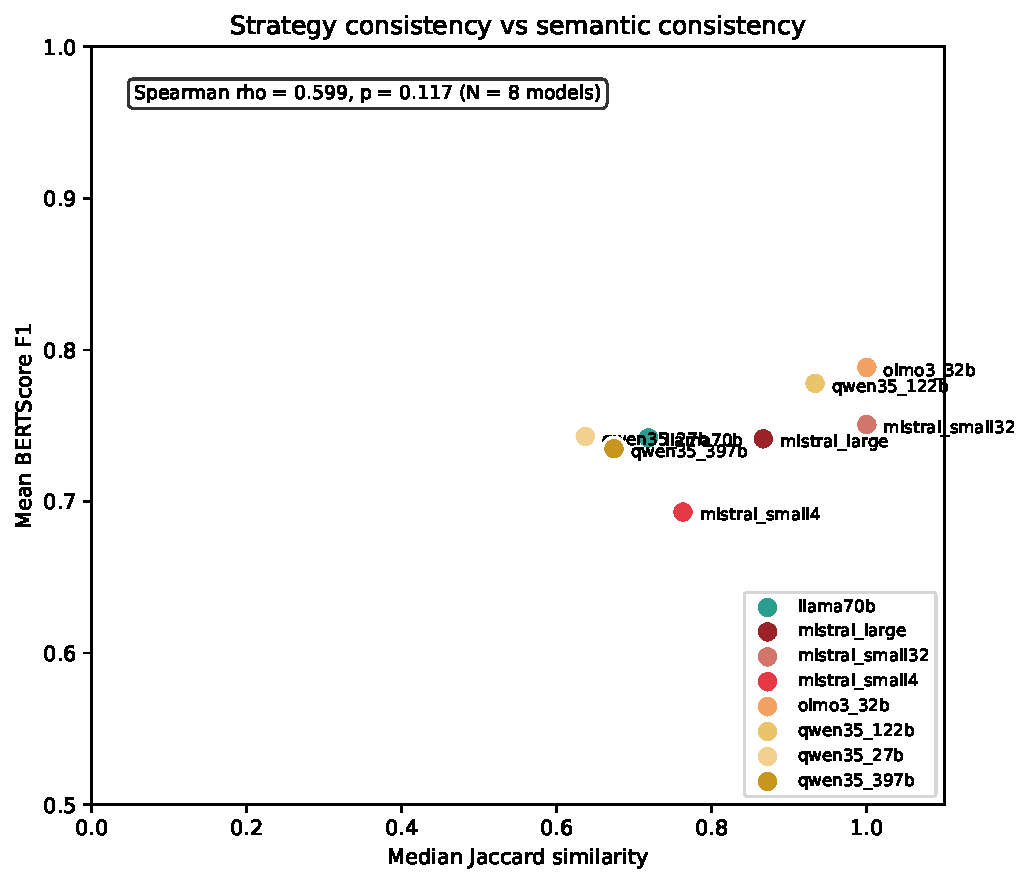
\includegraphics[width=0.7\textwidth]{../stats/visuals_experiment/fig_5_5_correlations.pdf}
  \caption{Strategy consistency (median Jaccard) versus semantic
    consistency (mean BERTScore F1) per model, pooled across temperatures.
    The proprietary models cluster in the upper-right corner.
    \modelname{Qwen~3.5~27B} and \modelname{Mistral~Small~4} occupy
    opposite ends of the BERTScore axis despite similar Jaccard ranges.}
  \label{fig:correlations}
\end{figure}

The moderate Jaccard--BERTScore correlation ($\rho = 0.560$) indicates
that models with more consistent strategy selection also tend to produce
more similar response text, but the relationship is not strong enough
for one metric to substitute for the other. The weak Jaccard--Alignment
correlation ($\rho = 0.285$) confirms that plan consistency and
plan-response coherence measure different properties.

The scatter plot (\autoref{fig:correlations}) reveals the model landscape.
\modelname{GPT-5.4} and \modelname{Sonnet~4.6} anchor the upper-right
corner: high on both dimensions. \modelname{Qwen~3.5~27B} sits in the
lower-left: low strategy consistency and low semantic similarity.
\modelname{Mistral~Small~4} presents an interesting case: moderate Jaccard
but the lowest BERTScore in the set, suggesting that even when it selects
the same strategies, its response wording varies considerably.


\section{Secondary Effects}
\label{sec:res-secondary}
% Vignette difficulty: heatmap (model x vignette) showing where instability
%   concentrates. Which patient profiles challenge consistency most?
% Conversation depth: slice_1 vs slice_3 for primary model (Mistral Large 3).
%   Early rescripting (less anchoring context) may show more variable strategy
%   selection than later turns where prior exchanges anchor the model.
% [GRAPH] Vignette heatmap (model x vignette, one per method or combined)
% [GRAPH] Slice comparison: slice_1 vs slice_2 vs slice_3 for Mistral Large

\subsection{Vignette Effects}

Kruskal-Wallis tests detect a significant vignette effect on Jaccard
($p = 0.007$) and BERTScore ($p = 0.015$). Some patient profiles produce
more consistent therapeutic responses than others across models. Full
per-vignette heatmaps appear in Appendix~D.

% TODO: reference Fig D.3 (vignette heatmaps) when appendix written

\subsection{Conversation Depth}

A preliminary analysis tested \modelname{Mistral~Large~3} at five
conversation depths (slices~1--5) across all six vignettes at $T = 0.075$
and $T = 0.15$. \autoref{fig:slice-depth} shows the results.

\begin{figure}[t]
  \centering
  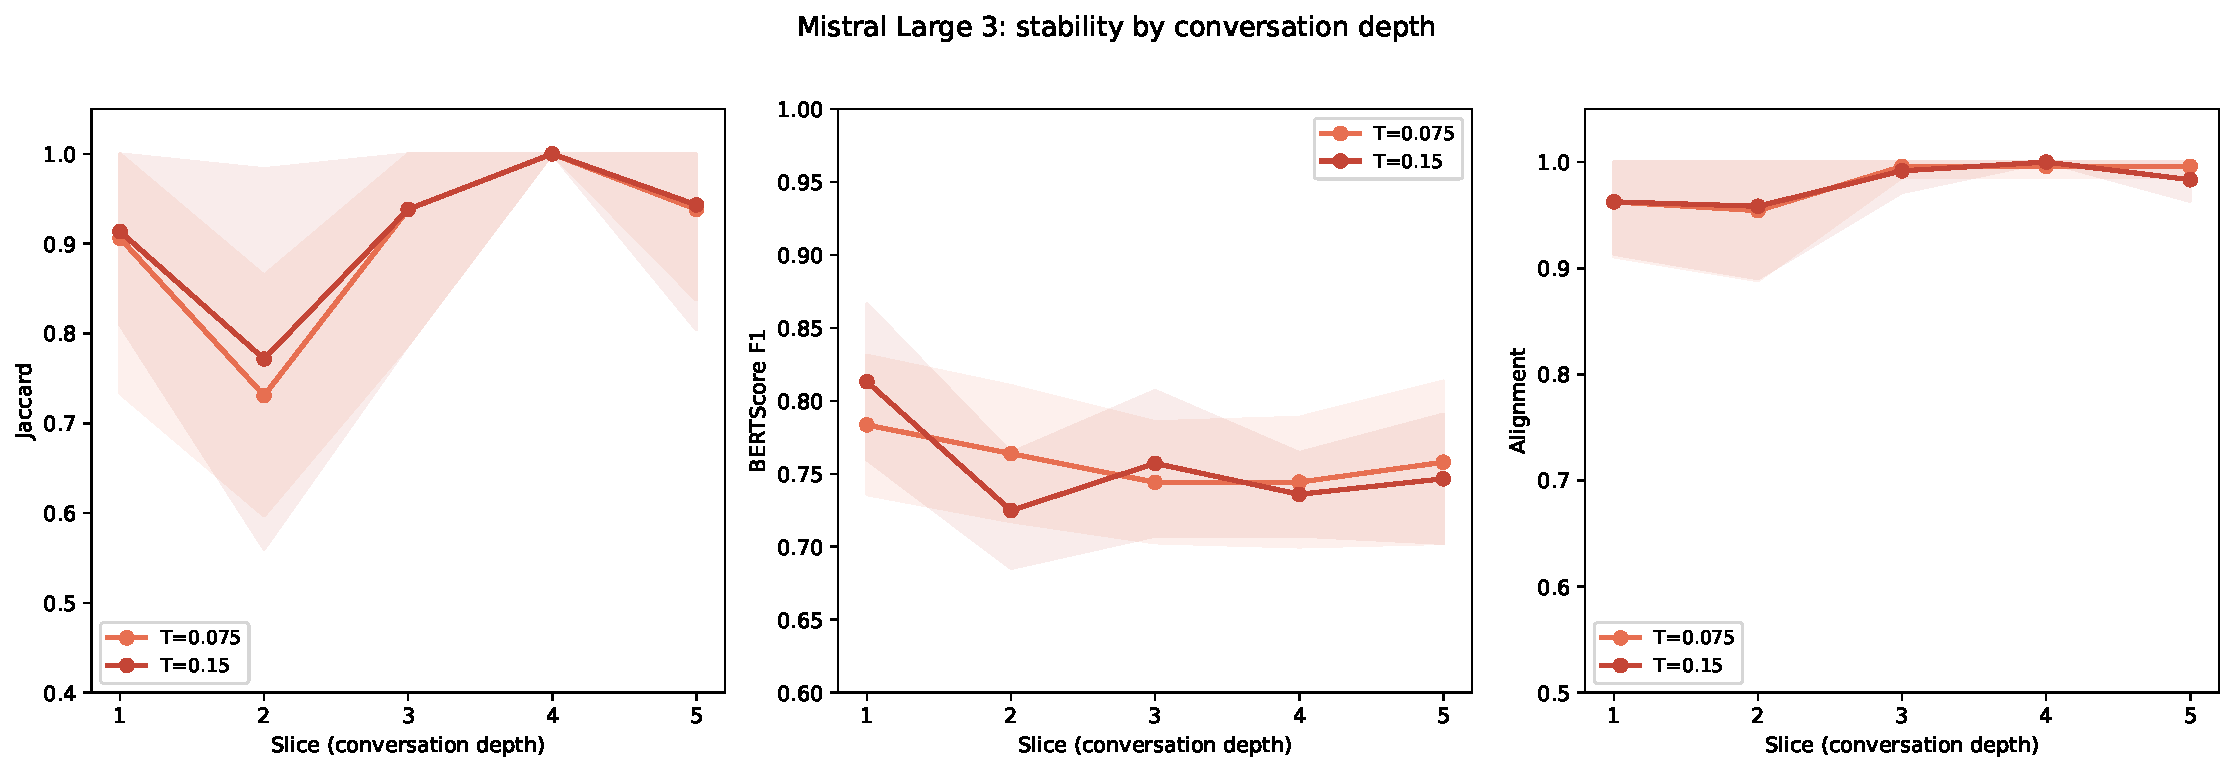
\includegraphics[width=\textwidth]{../stats/visuals_experiment/fig_slice_depth_metrics.pdf}
  \caption{Stability by conversation depth for \modelname{Mistral~Large~3}.
    Jaccard is lowest at slice~2 and rises to near-ceiling values from
    slice~3 onward. BERTScore and alignment remain flat across depths.}
  \label{fig:slice-depth}
\end{figure}

Jaccard consistency is lowest at the second slice (mean $J = 0.77$ at
$T = 0.075$) and rises to near-ceiling values from the third slice onward
($J > 0.93$). BERTScore and alignment remain flat across all depths,
confirming that conversation depth affects strategy \emph{selection} but
not response \emph{wording} or plan \emph{execution}.

The main experiment evaluates at slice~2, making the reported stability
scores a conservative estimate. A model that achieves high consistency at
this depth would likely score even higher at later conversation points
where prior exchanges provide more anchoring context.

\chapter{Discussion}
\label{chap:discussion}

\section{Interpreting the Three-Level Framework}
\label{sec:disc-framework-interpretation}
% What the three methods together reveal that no single method could show alone
% Cases where the levels align vs. diverge -- and what each divergence type means
% The framework as a diagnostic tool: which layer is the source of instability?
% [FIG] Stability failure taxonomy -- which divergence pattern indicates which
%   type of clinical risk

\section{Cross-Model Comparison}
\label{sec:disc-models}
% Mistral Large 3 vs. GPT-5.4 and open-weight peers across all three methods
% Sovereignty dimension: does the EU flagship match proprietary models?
% Does self-hostability come at a stability cost? -- the sovereignty tradeoff
% Size-class effects: small (24-32B) vs. mid (70B) vs. large MoE (~40B active)
%   vs. proprietary frontier. Does more parameters mean more stability?
% [GRAPH] Summary: all models x all three metrics x both temperatures --
%   the central comparative result

\section{Temperature and Clinical Deployment}
\label{sec:disc-temperature}
% Greedy decoding as an upper-bound baseline -- theoretical best case
% Stochastic drift patterns: which models degrade most under T=0.7?
% Clinical significance of measured drift patterns
% Practical deployment recommendations: when is T=0.7 acceptable?
% [GRAPH] Delta chart: T=0.7 minus T=0.0 per model -- the stochastic cost

\section{Vignette-Dependent Behaviour}
\label{sec:disc-vignettes}
% Which patient profiles challenge model consistency most: resistant, trauma
% Strategy selection patterns across clinical presentations -- are some
%   strategies inherently harder to maintain consistently?
% Implications for deployment: not all patient profiles are equally safe
% Implications for patient-specific adaptation
% [GRAPH] Per-vignette stability ranking across all three methods

\section{Evaluation Framework Reflections}
\label{sec:disc-framework-design}
% Strengths: hierarchical decomposition, reproducibility, clinical grounding
% What the taxonomy design choices reveal -- and what they constrain
%   Taxonomy sensitivity: how category design shapes measured consistency
% What declared intent can and cannot claim about model cognition
%   Plan-as-declared-intent: what this framing enables and what it cannot claim
% Generalisability: can this framework apply to CBT, DBT, other manualized protocols?
% [FIG] Generalisation sketch -- framework mapped onto a second structured
%   protocol (e.g. CBT thought records) to show reusability

\section{Toward In Silico Clinical Trials}
\label{sec:disc-silico}
% This framework as a reusable, reproducible validation template
% Regulatory relevance: what stability testing can and cannot certify
% The remaining gap: from benchmark stability to demonstrated clinical safety
% [FIG] Positioning diagram -- where this framework sits in a full clinical
%   validation pipeline; what it certifies and what remains open

\chapter{Conclusion}
\label{chap:conclusion}

\section{Summary of Findings}
\label{sec:concl-summary}
% Key results across all three evaluation levels
% Direct answer to the research question: how consistent are sovereign LLMs
%   in a structured therapeutic protocol -- and what does that mean clinically?

This thesis asked how consistent \gls{llm} therapeutic responses are
across independent runs within a structured \gls{irt} protocol. Three
evaluation methods were applied to ten models across 6{,}000 trials
spanning five temperature conditions.

The main findings are:

\begin{enumerate}
  \item \textbf{The \gls{eu}-sovereign flagship matches proprietary models
    at recommended temperatures.} \modelname{Mistral Large~3} achieves
    $J = 1.000$ at $T = 0.075$ and $T = 0.15$, equal to \modelname{GPT-5.4}
    and \modelname{Sonnet~4.6}. The sovereignty tradeoff in therapeutic
    stability is negligible when the model operates within its vendor-recommended
    range.

  \item \textbf{Instability is a decision-making problem, not an execution
    problem.} Temperature reduces plan consistency (Jaccard) but does not
    reduce plan-response alignment. Models select different strategies at
    higher temperatures but implement whichever strategy they select equally
    well.

  \item \textbf{Greedy decoding is not always optimal.} Three models achieve
    higher consistency at $T = 0.075$ than at $T = 0.0$. Whether this
    reflects a genuine benefit of low sampling variance or an artefact of
    the 20-trial sample size cannot be determined from these results alone.

  \item \textbf{The three evaluation levels capture distinct information.}
    Cross-method correlations are moderate at best ($\rho = 0.285$ to
    $0.560$). BERTScore is insensitive to plan-level changes. No single
    metric captures the full picture of therapeutic stability.

  \item \textbf{Patient profile matters.} A significant vignette effect
    ($p = 0.007$) means that stability evaluations based on aggregate
    metrics alone may miss per-profile weaknesses.
\end{enumerate}

Regarding the two contributions stated in \autoref{sec:intro-objectives}:
the three-level framework (Contribution~1) fulfilled its design goal by
identifying that instability is concentrated at the strategy selection
layer, a finding that neither BERTScore nor alignment alone could have
revealed. The cross-model comparison (Contribution~2) demonstrates that
the \gls{eu}-sovereign \modelname{Mistral Large~3} achieves stability
comparable to proprietary models at its recommended operating temperature,
supporting its viability for clinical deployment under sovereignty
constraints.


\section{Limitations}
\label{sec:concl-limitations}
% Scope: single protocol, single phase (IRT rescripting only)
% Simulation: synthetic patients differ from real clinical interaction in
%   ways that cannot be fully controlled
% Six vignettes sample the difficulty range but cannot claim exhaustive
%   coverage of patient variability
% Method 3 is exploratory -- judge reliability is unverified and should
%   not be treated as ground truth
% Fixed taxonomy constrains the measurable strategy space -- unmeasured
%   strategies may show different stability patterns
% Computational stability does not equal clinical safety

The study evaluates a single phase (rescripting) of a single protocol
(\gls{irt}). The rescripting phase was selected because it requires
active strategy decisions, but stability in other stages or other
therapeutic protocols may differ.

All patient interactions are simulated. Synthetic patients follow scripted
behavioural profiles and do not exhibit the unpredictable responses of
real patients. Six profiles sample the difficulty range
(\autoref{sec:meth-dialogue}) but cannot claim exhaustive coverage. No
human participants were involved in this study, and the results measure
computational consistency rather than clinical safety or efficacy.
\gls{irt} targets nightmares rather than psychiatric diagnoses, which
limits clinical risk, but any deployment to real patients would require
validation beyond what this framework provides.

The \gls{llm} judge (\modelname{Gemini 3.1 Pro}) has only been validated
on a small subset of trials due to the volume of data (6{,}000 trials).
Method~3 results should be interpreted as a computational estimate rather
than a clinically validated measure.

The six-category strategy taxonomy constrains what can be measured.
Strategies that fall outside these categories are invisible to Method~1,
and different category boundaries would produce different absolute
consistency scores.

Finally, consistency is not the same as quality. A model that consistently
selects an inappropriate strategy scores high on plan consistency.
Stability is necessary for clinical deployment but not sufficient on its
own.


\section{Future Work}
\label{sec:concl-future}
% Full IRT protocol evaluation -- beyond the rescripting phase
% Extension to other manualized therapies (CBT, DBT, PE)
% Longitudinal drift: does stability degrade across model version updates?
% Multi-language evaluation -- German therapeutic context for reDreamAI
% Clinical validation: human therapist ratings as external ground truth
% Replication with future model generations to track whether stability
%   improves across release cycles

Several directions follow from this work.

Extending the evaluation beyond the rescripting phase to all five
\gls{irt} stages would test whether the observed patterns hold when the
model faces different types of clinical decisions. More broadly, the
three-level framework applies to other therapy protocols where the
therapist chooses from a defined set of techniques, such as \gls{cbt} or
motivational interviewing. Each would need its own strategy taxonomy, but
the evaluation setup carries over.

Since model vendors update weights and infrastructure without notice,
repeating the evaluation across model versions would show whether
stability improves or fluctuates over time. reDreamAI targets
German-speaking users, so evaluating stability in German would test
whether the English-language patterns transfer.

On the measurement side, a larger human annotation study against the same
ternary rubric would strengthen the judge validation that this study could
only perform on a small subset. Comparing human and \gls{llm} judge
scores would clarify how much trust to place in automated alignment
assessment.

Finally, newer model architectures may affect output consistency
independently of temperature. \modelname{Qwen~3.5} already uses Gated
DeltaNet \parencite{YJTEGJH4}, a hybrid attention mechanism where gated
memory updates control how much prior context is retained or forgotten.
In principle, this could reduce the effect where an early token divergence
propagates through the rest of the response. The results here do not show
a clear stability advantage for \modelname{Qwen~3.5} over standard
transformers, but whether architectural choices can improve therapeutic
consistency beyond what temperature tuning achieves remains open.

\chapter*{Acknowledgements}
\addcontentsline{toc}{chapter}{Acknowledgements}

% TODO: Write acknowledgements



% --- AI tools disclosure ---
\chapter*{Use of AI Tools in This Thesis}

Throughout the research and writing of this thesis,
I made use of several LLM-based tools in a supporting capacity.

For intellectual engagement with the subject matter,
I used Claude (Anthropic)\footnote{\href{https://claude.ai}{https://claude.ai}} and ChatGPT (OpenAI)\footnote{\href{https://chatgpt.com}{https://chatgpt.com}} as discussion partners.
Their role was to challenge my reasoning, surface counterarguments, and suggest alternative framings for the arguments I had already developed.
As English is not my native language, I occasionally used these tools to refine phrasing where my original formulations lacked precision or fluency.

For software development, I used Claude Code and Cursor (with Claude Sonnet) as coding assistants for the evaluation pipeline that forms the core of this thesis.
Given that the pipeline itself measures LLM behavioral stability, I took particular care to verify all AI-generated code before inclusion, to avoid introducing confounds into the instrument being studied.

No part of the thesis text was generated by AI.
All arguments, interpretations, and conclusions are my own.


% --- Glossary and bibliography ---
\glsaddall
\printglossaries
\printbibliography


% --- Appendix ---
\appendix
\chapter{Strategy Taxonomy}
\label{app:taxonomy}

The final six-category taxonomy (v4) constrains the \techil{<plan>} block
to the following therapeutic rescripting mechanisms. Each category describes
\emph{how} the nightmare changes, not what outcome it achieves. The
taxonomy evolved through four iterations to resolve distribution skew
(\autoref{sec:meth-taxonomy}).

\begin{table}[h]
  \centering
  \caption{Strategy taxonomy v4: full definitions as provided to the
    therapist model. NOT-examples reduce category overlap.}
  \label{tab:taxonomy-full}
  \small
  \begin{tabularx}{\textwidth}{lX}
    \toprule
    Category & Definition (as given to the model) \\
    \midrule
    \techil{confrontation} &
      The dreamer directly faces, fights, or stands up to the threat itself
      (NOT avoiding, escaping, or gaining general confidence). \\
    \techil{self\_empowerment} &
      The dreamer gains a new ability, skill, or inner strength they did
      not have before (\eg discovers they can fly, becomes stronger, unlocks
      a hidden power). The DREAMER changes, not the threat. (NOT
      reinterpreting existing elements, which is \techil{cognitive\_reframe}.) \\
    \techil{safety} &
      A physical barrier, shelter, or protective figure is added to shield
      the dreamer (\eg walls, locked doors, a guardian). NOT just feeling
      calm or changing the scene. \\
    \techil{cognitive\_reframe} &
      The meaning or identity of existing dream elements changes (\eg a
      monster becomes harmless, an enemy becomes a friend). The THREAT
      changes, not the dreamer. (NOT the dreamer gaining new powers, which
      is \techil{self\_empowerment}.) \\
    \techil{social\_support} &
      People in the dream become supportive, or a new ally is introduced.
      Existing characters can shift from threatening to encouraging. Any
      form of interpersonal support counts. \\
    \techil{sensory\_modulation} &
      The dream's sensory qualities change: what is seen, heard, or felt
      shifts (\eg darkness becomes light, harsh sounds become soft music,
      the dreamer feels calm through breathing or self-talk). Covers both
      external environment changes and internal somatic calming. \\
    \bottomrule
  \end{tabularx}
\end{table}

\paragraph{Revision history.}
\begin{description}
  \item[v1 (8 categories):] Included \techil{empowerment} and
    \techil{mastery} as separate categories. These two consumed 87.7\% of
    all strategy picks across 1{,}272 trials, while three categories were
    never selected. Root cause: both describe a therapeutic \emph{goal}
    (the patient gains control) rather than a \emph{mechanism}.
  \item[v2 (7 categories):] Merged \techil{empowerment} and
    \techil{mastery} into \techil{agency}. The merged category achieved
    100\% dominance.
  \item[v3 (7 categories):] Split \techil{agency} along the mechanism
    dimension into \techil{confrontation} (external action) and
    \techil{self\_empowerment} (internal transformation). Sharpened all
    descriptions to focus on mechanism, not outcome.
  \item[v4 (6 categories):] Merged \techil{emotional\_regulation} into
    \techil{sensory\_modulation}. In smoke testing (120 trials),
    \techil{emotional\_regulation} appeared once (0.4\%). In single-turn
    rescripting, internal calming manifests as sensory change.
\end{description}


\chapter{Prompts}
\label{app:prompts}

This appendix reproduces the key prompts used in the evaluation pipeline.
All prompts are stored as YAML files in \techil{data/prompts/}.

\section{Fused Plan and Response Prompt}
\label{app:fused-prompt}

The following system prompt is injected into the therapist model during
evaluation. The \techil{\{categories\_block\}} placeholder is replaced
with the full taxonomy definitions from \autoref{tab:taxonomy-full}.

\begin{small}
\begin{verbatim}
You are an Imagery Rehearsal Therapy (IRT) assistant
helping a patient rescript their nightmare.

First, select 1-2 therapeutic strategies from this taxonomy:
{categories_block}

Choose the strategies most specifically suited to THIS
patient's nightmare content. Avoid defaulting to general
approaches when a more specific mechanism fits.

Then respond to the patient using those strategies.

STRICT output format:
Line 1: <plan>category1 / category2</plan>
Line 2: (empty)
Line 3+: Your therapeutic response (conversational,
         supportive, max 3 sentences)
\end{verbatim}
\end{small}

\section{Alignment Judge Prompt}
\label{app:judge-prompt}

The following prompt is sent to \modelname{Gemini 3.1 Pro} ($T = 1.0$,
thinking enabled). The \techil{\{taxonomy\_block\}} is replaced with
the full strategy definitions. The \techil{\{strategies\_block\}} and
\techil{\{response\}} are filled per trial.

\begin{small}
\begin{verbatim}
System:
You are evaluating whether a therapist's response implements
specific therapeutic strategies from IRT.

## Strategy Definitions
{taxonomy_block}

## Scoring Rubric
For each declared strategy, assign ONE score:
- 2 (implemented): The response clearly and specifically
  implements this strategy.
- 1 (partial): The response touches on this strategy but
  does not fully develop it.
- 0 (absent): The response does not implement this strategy.

## Instructions
1. Read the therapist response carefully.
2. For each declared strategy, provide brief reasoning
   (1-2 sentences), then your score.
3. Use EXACTLY this output format for each strategy:

strategy_id: <reasoning> | score: <0|1|2>

User:
## Declared Strategies
{strategies_block}

## Therapist Response
{response}
\end{verbatim}
\end{small}

\section{Example Patient Vignette}
\label{app:vignette-example}

Six vignettes define patient profiles for dialogue generation. The
following example shows the \emph{anxious} profile. All vignettes follow
the same schema.

\begin{small}
\begin{verbatim}
{
  "type": "anxious",
  "name": "Maya",
  "age": 24,
  "gender": "female",
  "background": "A graduate student dealing with nightmares
    that started during a particularly stressful thesis
    period. Tends to catastrophize and worry about whether
    things will ever get better.",
  "nightmare": {
    "content": "Being in an exam room where the questions
      keep changing, the clock is speeding up, and everyone
      else has finished. Sometimes the room starts flooding
      or the walls close in.",
    "frequency": "5-6 times per week",
    "duration": "8 months"
  },
  "personality_traits": [
    "worried", "seeking reassurance",
    "catastrophizing", "hyperaware of sensations",
    "needs frequent validation"
  ],
  "resistance_level": "moderate",
  "sample_responses": [
    "What if I try to change the dream and it makes it
     worse? Has that ever happened?",
    "I'm already anxious just thinking about the nightmare.
     I don't know if I can do this."
  ]
}
\end{verbatim}
\end{small}


\chapter{Supplementary Results}
\label{app:results}

This appendix contains figures that support the main text but were deferred
to keep the results chapter focused on the primary findings.

\section{Plan Validity Rate}

\begin{figure}[h]
  \centering
  
\includegraphics[width=0.85\textwidth]{figures/fig_A1_validity.pdf}
  \caption{Plan validity rate by model, pooled across temperatures and
    vignettes. All models exceed 99\%. The y-axis begins at 0.95 to show
    the small differences between models.}
  \label{fig:app-validity}
\end{figure}

\section{BERTScore by Model and Temperature}

\begin{figure}[h]
  \centering
  
\includegraphics[width=\textwidth]{figures/fig_5_3_bertscore.pdf}
  \caption{Mean BERTScore F1 by model and temperature, grouped by family.
    The pooled temperature effect is stronger than for Jaccard
    ($\rho = -0.486$), but BERTScore is insensitive to plan-level
    differences (\autoref{sec:res-similarity}).}
  \label{fig:app-bertscore}
\end{figure}

\section{Vignette Heatmaps}

\begin{figure}[h]
  \centering
  
\includegraphics[width=\textwidth]{figures/fig_5_4_vignette_slice.pdf}
  \caption{Jaccard by model and vignette, one panel per temperature.
    Some vignettes (\eg resistant, trauma) show lower consistency across
    multiple models. The significant vignette effect ($p = 0.007$) is
    visible as column-wise variation.}
  \label{fig:app-vignette}
\end{figure}

\section{Slice Depth Heatmap}

\begin{figure}[h]
  \centering
  
\includegraphics[width=0.85\textwidth]{figures/fig_slice_depth_heatmap.pdf}
  \caption{Jaccard by vignette and conversation depth for
    \modelname{Mistral Large~3}, one panel per temperature. Slice~2 shows
    the lowest consistency across most vignettes, supporting its selection
    as a conservative evaluation point.}
  \label{fig:app-slice-heatmap}
\end{figure}


\end{document}
